%%%%%%%%%%%%%%%%%%%%%%%%%%%%
% Two Sword Lengths Apart: Supplementary Material
% 20 March 2014
%%%%%%%%%%%%%%%%%%%%%%%%%%%%

% !Rnw weave = knitr

\documentclass[a4paper]{article}\usepackage[]{graphicx}\usepackage[]{color}
%% maxwidth is the original width if it is less than linewidth
%% otherwise use linewidth (to make sure the graphics do not exceed the margin)
\makeatletter
\def\maxwidth{ %
  \ifdim\Gin@nat@width>\linewidth
    \linewidth
  \else
    \Gin@nat@width
  \fi
}
\makeatother

\definecolor{fgcolor}{rgb}{0.345, 0.345, 0.345}
\newcommand{\hlnum}[1]{\textcolor[rgb]{0.686,0.059,0.569}{#1}}%
\newcommand{\hlstr}[1]{\textcolor[rgb]{0.192,0.494,0.8}{#1}}%
\newcommand{\hlcom}[1]{\textcolor[rgb]{0.678,0.584,0.686}{\textit{#1}}}%
\newcommand{\hlopt}[1]{\textcolor[rgb]{0,0,0}{#1}}%
\newcommand{\hlstd}[1]{\textcolor[rgb]{0.345,0.345,0.345}{#1}}%
\newcommand{\hlkwa}[1]{\textcolor[rgb]{0.161,0.373,0.58}{\textbf{#1}}}%
\newcommand{\hlkwb}[1]{\textcolor[rgb]{0.69,0.353,0.396}{#1}}%
\newcommand{\hlkwc}[1]{\textcolor[rgb]{0.333,0.667,0.333}{#1}}%
\newcommand{\hlkwd}[1]{\textcolor[rgb]{0.737,0.353,0.396}{\textbf{#1}}}%

\usepackage{framed}
\makeatletter
\newenvironment{kframe}{%
 \def\at@end@of@kframe{}%
 \ifinner\ifhmode%
  \def\at@end@of@kframe{\end{minipage}}%
  \begin{minipage}{\columnwidth}%
 \fi\fi%
 \def\FrameCommand##1{\hskip\@totalleftmargin \hskip-\fboxsep
 \colorbox{shadecolor}{##1}\hskip-\fboxsep
     % There is no \\@totalrightmargin, so:
     \hskip-\linewidth \hskip-\@totalleftmargin \hskip\columnwidth}%
 \MakeFramed {\advance\hsize-\width
   \@totalleftmargin\z@ \linewidth\hsize
   \@setminipage}}%
 {\par\unskip\endMakeFramed%
 \at@end@of@kframe}
\makeatother

\definecolor{shadecolor}{rgb}{.97, .97, .97}
\definecolor{messagecolor}{rgb}{0, 0, 0}
\definecolor{warningcolor}{rgb}{1, 0, 1}
\definecolor{errorcolor}{rgb}{1, 0, 0}
\newenvironment{knitrout}{}{} % an empty environment to be redefined in TeX

\usepackage{alltt}
\usepackage{fullpage}
\usepackage{lscape}
\usepackage[authoryear]{natbib}
\usepackage{setspace}
    \doublespacing
\usepackage{hyperref}
\hypersetup{
    colorlinks,
    citecolor=black,
    filecolor=black,
    linkcolor=cyan,
    urlcolor=cyan
}
\usepackage{booktabs}
\usepackage{dcolumn}
\usepackage{url}
\usepackage{tikz}
\usepackage{todonotes}
\usepackage{verbatim}
\usepackage{endnotes}
\usepackage{graphicx}

\usepackage[margins]{trackchanges}

\usepackage{footmisc}
\setlength{\footnotesep}{\baselineskip}
\renewcommand{\footnotelayout}{\doublespacing\normalsize}

\setlength{\belowcaptionskip}{0.5cm}

%%%%%%% Title Page %%%%%%%%%%%%%%%%%%%%%%%%%%%%%%%%%%%%%%%%%%%%
\title{Supplementary Material: Two Sword Lengths Apart: Credible Commitment Problems and Physical Violence in Multi-party Elected National Legislatures}
\IfFileExists{upquote.sty}{\usepackage{upquote}}{}
\begin{document}

\maketitle



%%%%%%%%%%%%%%%% Run Analyses %%%%%%%%%%%%%%%%%%%%%%%%



\subsection*{Details on Prior Correction of the Rare Logistic Regression Models}

For prior correction \citep[see][]{KingRareEventsPA2001} in the models with the full sample of elected multi-party legislatures I used the observed proportion of all observations with legislative violence \change{up to 2010}{through 2012}: i.e. \change{2.1}{2.2} percent of observations up until 2010 had violence ($\tau = \frac{117}{5360} = 0.022$). There were \change{63}{109} observed incidences of violence and \change{2654}{3990} country-years from 1990 through \change{2009}{2012} in the sample, so: $\tau = \frac{109}{3390} = 0.027$.

%%%%%%%% Elected Legislatures Results Table
\begin{table}
\caption{Legislative Violence Rare Events Logistic Regression Results (Multi-Party Elected Legislature 1981-2012)}
\label{outputTable.dem}
\begin{center}
{\scalebox{0.65}{

% Table created by stargazer v.5.1 by Marek Hlavac, Harvard University. E-mail: hlavac at fas.harvard.edu
% Date and time: Fri, Mar 20, 2015 - 15:02:56
\begin{tabular}{@{\extracolsep{5pt}}lcccccccccc} 
\\[-1.8ex]\hline 
\hline \\[-1.8ex] 
 & \multicolumn{10}{c}{\textit{Dependent variable:}} \\ 
\cline{2-11} 
\\[-1.8ex] & \multicolumn{10}{c}{Violent Incident} \\ 
\\[-1.8ex] & (1) & (2) & (3) & (4) & (5) & (6) & (7) & (8) & (9) & (10)\\ 
\hline \\[-1.8ex] 
 Low Disproportionality & $-$0.572$^{**}$ & $-$0.551$^{**}$ & $-$0.825$^{***}$ & $-$0.419 & $-$0.667$^{**}$ & $-$0.400 & $-$0.605$^{**}$ & $-$0.522$^{**}$ & $-$0.522$^{**}$ & $-$0.416 \\ 
  & (0.249) & (0.250) & (0.258) & (0.280) & (0.292) & (0.352) & (0.257) & (0.254) & (0.251) & (0.261) \\ 
  & & & & & & & & & & \\ 
 Dem. Age & $-$0.011$^{**}$ & $-$0.011$^{**}$ & $-$0.012$^{**}$ & $-$0.017$^{***}$ & $-$0.010$^{**}$ & $-$0.012$^{*}$ & $-$0.017$^{***}$ & $-$0.015$^{***}$ & $-$0.015$^{***}$ & $-$0.016$^{**}$ \\ 
  & (0.005) & (0.005) & (0.005) & (0.006) & (0.005) & (0.007) & (0.005) & (0.005) & (0.005) & (0.007) \\ 
  & & & & & & & & & & \\ 
 Majority Size & $-$0.030$^{***}$ & $-$0.030$^{***}$ & $-$0.029$^{***}$ & $-$0.031$^{***}$ & $-$0.028$^{***}$ & $-$0.015 & $-$0.028$^{***}$ & $-$0.029$^{***}$ & $-$0.032$^{***}$ & $-$0.029$^{***}$ \\ 
  & (0.008) & (0.008) & (0.008) & (0.010) & (0.009) & (0.012) & (0.008) & (0.009) & (0.008) & (0.008) \\ 
  & & & & & & & & & & \\ 
 Internal Armed Conflict &  & 0.782$^{***}$ & 0.704$^{***}$ & 0.760$^{**}$ & 0.817$^{***}$ & 0.776$^{*}$ & 0.752$^{***}$ & 0.846$^{***}$ & 0.899$^{***}$ & 1.000$^{***}$ \\ 
  &  & (0.267) & (0.270) & (0.318) & (0.302) & (0.415) & (0.276) & (0.274) & (0.273) & (0.284) \\ 
  & & & & & & & & & & \\ 
 Leg. Immunity &  &  & $-$0.263 &  &  &  &  &  &  &  \\ 
  &  &  & (0.255) &  &  &  &  &  &  &  \\ 
  & & & & & & & & & & \\ 
 PR Electoral System &  &  & 1.452$^{***}$ &  &  &  &  &  &  &  \\ 
  &  &  & (0.452) &  &  &  &  &  &  &  \\ 
  & & & & & & & & & & \\ 
 Single Party Gov. &  &  & $-$0.248 &  &  &  &  &  &  &  \\ 
  &  &  & (0.243) &  &  &  &  &  &  &  \\ 
  & & & & & & & & & & \\ 
 Self Expression &  &  &  & 2.334 &  &  &  &  &  &  \\ 
  &  &  &  & (2.290) &  &  &  &  &  &  \\ 
  & & & & & & & & & & \\ 
 Ethnic Frac. &  &  &  & $-$0.973 &  &  &  &  &  &  \\ 
  &  &  &  & (0.728) &  &  &  &  &  &  \\ 
  & & & & & & & & & & \\ 
 Perc. Women in Parl. &  &  &  &  & 0.010 &  &  &  &  &  \\ 
  &  &  &  &  & (0.015) &  &  &  &  &  \\ 
  & & & & & & & & & & \\ 
 Murder Rate &  &  &  &  &  & $-$0.001 &  &  &  &  \\ 
  &  &  &  &  &  & (0.012) &  &  &  &  \\ 
  & & & & & & & & & & \\ 
 Federal &  &  &  &  &  &  & 0.605$^{*}$ &  &  &  \\ 
  &  &  &  &  &  &  & (0.313) &  &  &  \\ 
  & & & & & & & & & & \\ 
 Gov. Frac. &  &  &  &  &  &  & 0.109 &  &  &  \\ 
  &  &  &  &  &  &  & (0.434) &  &  &  \\ 
  & & & & & & & & & & \\ 
 No. of Parties by Seats &  &  &  &  &  &  &  & $-$0.053 &  &  \\ 
  &  &  &  &  &  &  &  & (0.079) &  &  \\ 
  & & & & & & & & & & \\ 
 GINI &  &  &  &  &  &  &  &  & $-$0.048$^{***}$ &  \\ 
  &  &  &  &  &  &  &  &  & (0.015) &  \\ 
  & & & & & & & & & & \\ 
 GDP per Capita &  &  &  &  &  &  &  &  &  & 0.019 \\ 
  &  &  &  &  &  &  &  &  &  & (0.018) \\ 
  & & & & & & & & & & \\ 
 (Intercept) & $-$1.333$^{***}$ & $-$1.468$^{***}$ & $-$2.358$^{***}$ & $-$3.932 & $-$1.685$^{***}$ & $-$2.165$^{***}$ & $-$1.558$^{***}$ & $-$1.261$^{**}$ & 0.606 & $-$1.686$^{***}$ \\ 
  & (0.436) & (0.443) & (0.636) & (2.867) & (0.528) & (0.686) & (0.478) & (0.622) & (0.767) & (0.482) \\ 
  & & & & & & & & & & \\ 
\hline \\[-1.8ex] 
Observations & 1,941 & 1,941 & 1,846 & 965 & 1,792 & 988 & 1,662 & 1,697 & 1,878 & 1,864 \\ 
Log Likelihood & $-$308.268 & $-$304.556 & $-$288.874 & $-$213.419 & $-$247.829 & $-$148.022 & $-$276.202 & $-$283.482 & $-$295.120 & $-$274.209 \\ 
Akaike Inf. Crit. & 624.537 & 619.112 & 593.749 & 440.837 & 507.658 & 308.045 & 566.404 & 578.965 & 602.240 & 560.419 \\ 
\hline 
\hline \\[-1.8ex] 
\textit{Note:}  & \multicolumn{10}{l}{$^{*}$p$<$0.1; $^{**}$p$<$0.05; $^{***}$p$<$0.01} \\ 
 & \multicolumn{10}{l}{Standard errors are in parentheses. All models use robust (WEAVE) standard errors.} \\ 
\end{tabular} 

}}
\end{center}

\end{table}

%%%%%%%% Elected Legislatures Results Table from 1990--Robustness
\begin{table}
\caption{Legislative Violence Regression Results (Multi-Party Elected Legislature from 1990-2012)}
\label{outputTable.1990}
\begin{center}
\scalebox{0.7}{

% Table created by stargazer v.5.1 by Marek Hlavac, Harvard University. E-mail: hlavac at fas.harvard.edu
% Date and time: Fri, Mar 20, 2015 - 15:03:00
\begin{tabular}{@{\extracolsep{5pt}}lcccccc} 
\\[-1.8ex]\hline 
\hline \\[-1.8ex] 
 & \multicolumn{6}{c}{\textit{Dependent variable:}} \\ 
\cline{2-7} 
\\[-1.8ex] & \multicolumn{6}{c}{Violent Incident} \\ 
\\[-1.8ex] & (1) & (2) & (3) & (4) & (5) & (6)\\ 
\hline \\[-1.8ex] 
 Low Disproportionality & $-$0.542$^{*}$ & $-$0.400 & $-$0.548$^{**}$ & $-$0.472$^{*}$ & $-$0.439$^{*}$ & $-$0.327 \\ 
  & (0.297) & (0.352) & (0.261) & (0.258) & (0.256) & (0.267) \\ 
  & & & & & & \\ 
 Dem. Age & $-$0.010$^{*}$ & $-$0.012$^{*}$ & $-$0.016$^{***}$ & $-$0.015$^{***}$ & $-$0.015$^{***}$ & $-$0.020$^{**}$ \\ 
  & (0.005) & (0.007) & (0.006) & (0.005) & (0.005) & (0.008) \\ 
  & & & & & & \\ 
 Majority Size & $-$0.027$^{***}$ & $-$0.015 & $-$0.026$^{***}$ & $-$0.029$^{***}$ & $-$0.031$^{***}$ & $-$0.029$^{***}$ \\ 
  & (0.009) & (0.012) & (0.009) & (0.009) & (0.008) & (0.009) \\ 
  & & & & & & \\ 
 Internal Armed Conflict & 0.674$^{**}$ & 0.776$^{*}$ & 0.684$^{**}$ & 0.793$^{***}$ & 0.889$^{***}$ & 0.976$^{***}$ \\ 
  & (0.332) & (0.415) & (0.303) & (0.300) & (0.298) & (0.309) \\ 
  & & & & & & \\ 
 Perc. Women in Parliament & 0.003 &  &  &  &  &  \\ 
  & (0.016) &  &  &  &  &  \\ 
  & & & & & & \\ 
 Murder Rate &  & $-$0.001 &  &  &  &  \\ 
  &  & (0.012) &  &  &  &  \\ 
  & & & & & & \\ 
 Federal &  &  & 0.474 &  &  &  \\ 
  &  &  & (0.343) &  &  &  \\ 
  & & & & & & \\ 
 Gov. Frac. &  &  & 0.037 &  &  &  \\ 
  &  &  & (0.454) &  &  &  \\ 
  & & & & & & \\ 
 No. of Parties by Seats &  &  &  & $-$0.072 &  &  \\ 
  &  &  &  & (0.082) &  &  \\ 
  & & & & & & \\ 
 Gini &  &  &  &  & $-$0.054$^{***}$ &  \\ 
  &  &  &  &  & (0.015) &  \\ 
  & & & & & & \\ 
 GDP per Capita &  &  &  &  &  & 0.032$^{*}$ \\ 
  &  &  &  &  &  & (0.019) \\ 
  & & & & & & \\ 
 (Intercept) & $-$1.690$^{***}$ & $-$2.165$^{***}$ & $-$1.629$^{***}$ & $-$1.238$^{*}$ & 0.709 & $-$1.774$^{***}$ \\ 
  & (0.546) & (0.686) & (0.486) & (0.643) & (0.793) & (0.499) \\ 
  & & & & & & \\ 
\hline \\[-1.8ex] 
Observations & 1,494 & 988 & 1,408 & 1,440 & 1,598 & 1,573 \\ 
Log Likelihood & $-$224.461 & $-$148.022 & $-$253.877 & $-$259.815 & $-$270.205 & $-$249.330 \\ 
Akaike Inf. Crit. & 460.922 & 308.045 & 521.755 & 531.631 & 552.410 & 510.660 \\ 
\hline 
\hline \\[-1.8ex] 
\textit{Note:}  & \multicolumn{6}{l}{$^{*}$p$<$0.1; $^{**}$p$<$0.05; $^{***}$p$<$0.01} \\ 
 & \multicolumn{6}{l}{Standard errors are in parentheses. All models use robust (WEAVE) standard errors.} \\ 
\end{tabular} 

}
\end{center}
{\scriptsize{
    Standard errors are in parentheses. All models use robust (WEAVE) standard errors. \\
}}
\end{table}



%%%%%%%%%%%%%%%%%%%%%% Figures Start %%%%%%%%%%%%%%%%%%%%%%%%%%%%%%%%%%%%%%%%%%%%%


%%%%%%%% Variable source summary table
\begin{table}[!h]
    \begin{center}
    \caption{Variable Summary}
    \label{var_summary}
    \begin{tabular}{l m{7cm} m{3.5cm}}

            \hline
            Variable & Description & Source \\
            \hline \hline
            Disprop & Gallagher Index of Electoral Disproportionality & \cite{Gallagher2012} \& \cite{Carey2011} \\
            ENPS & Effective number of parties by seats & \cite{Gallagher2012} \& \cite{Carey2011} \\
            ENPV & Effective number of parties by votes & \cite{Gallagher2012} \& \cite{Carey2011} \\
            Ethnic Fractionalization & Probability two randomly selected members of society are from the same ethnic group & \cite{Alesina2003} \\
            Federal & Whether a country has a federal system or not & \cite{Carey2011}, updated from 2003 by the author \\
            GDP/Capita & GDP per capita in thousands of US dollars & \cite{WorldBank2011} \\
            Gov. Fractionalization & Probability that two members of the Government will be from different parties & \cite{DPI2001} \\
            Gini & Gini Coefficient of income inequality & \cite{UNU2008} \\
            Immunity & Whether a legislators are immune from arrest and/or criminal prosecution or not & \cite{Fish2009} \\
            Internal Conflict & Internal armed conflict involving purely domestic as well as external combatants & UCDP/PRIO Armed Conflict Dataset \citep{Themner2014} \\
            LEIC & Legislative Indices of Electoral Competitiveness. Includes both the existence of a legislature and its level of electoral competitiveness. & \cite{DPI2001} \\
            Majority & Percentage of legislature controlled by governing parties & \cite{DPI2001} \\
            Murder Rate & Murders per 100,000 population & \cite{UNMurder2013} \\
            Polity & Polity IV Score & \cite{Marshall2009} \\
            PR & Whether a country uses a proportional representation electoral system or a plurality system & \cite{DPI2001} \\
            Self Expression & WVS self-expression indicator averaged across country-survey waves & \cite{WVS2009} \\
            System & Government system (parliamentary, presidential, or mixed & \cite{DPI2001} \\
            Tenshort & Tenure of the shortest serving veto player & \cite{DPI2001} \\
            Trust & Average of WVS responses where 1 $=$ most people can be trusted and 2 $=$ you can't be too careful & \cite{WVS2009} \\
            UDS & Posterior Mean Unified Democracy Score & \cite{Pemstein2010} \\
            Violence & Incidences of violence between legislators in the national parliamentary chamber & author \\
            Perc. Women in Parl. & Percentage of parliamentary seats held by women & \cite{WomParCrossNat} \& \cite{IPU2013} \\
            \hline

    \end{tabular}
    \end{center}
    \begin{singlespace}
        Please contact the author for detailed summary statistics. \\
        All of the data from \cite{DPI2001} was updated through 2012.
    \end{singlespace}
\end{table}

%%%%%%%%%% Correlation matrix %%%%%%%%%%
\begin{landscape}
\begin{figure}[t]
    \caption{Correlation Matrix for Variables Included in the Analysis (Multi-Party Elected Legislatures)}
    \label{corrmatrix}
    \begin{center}

    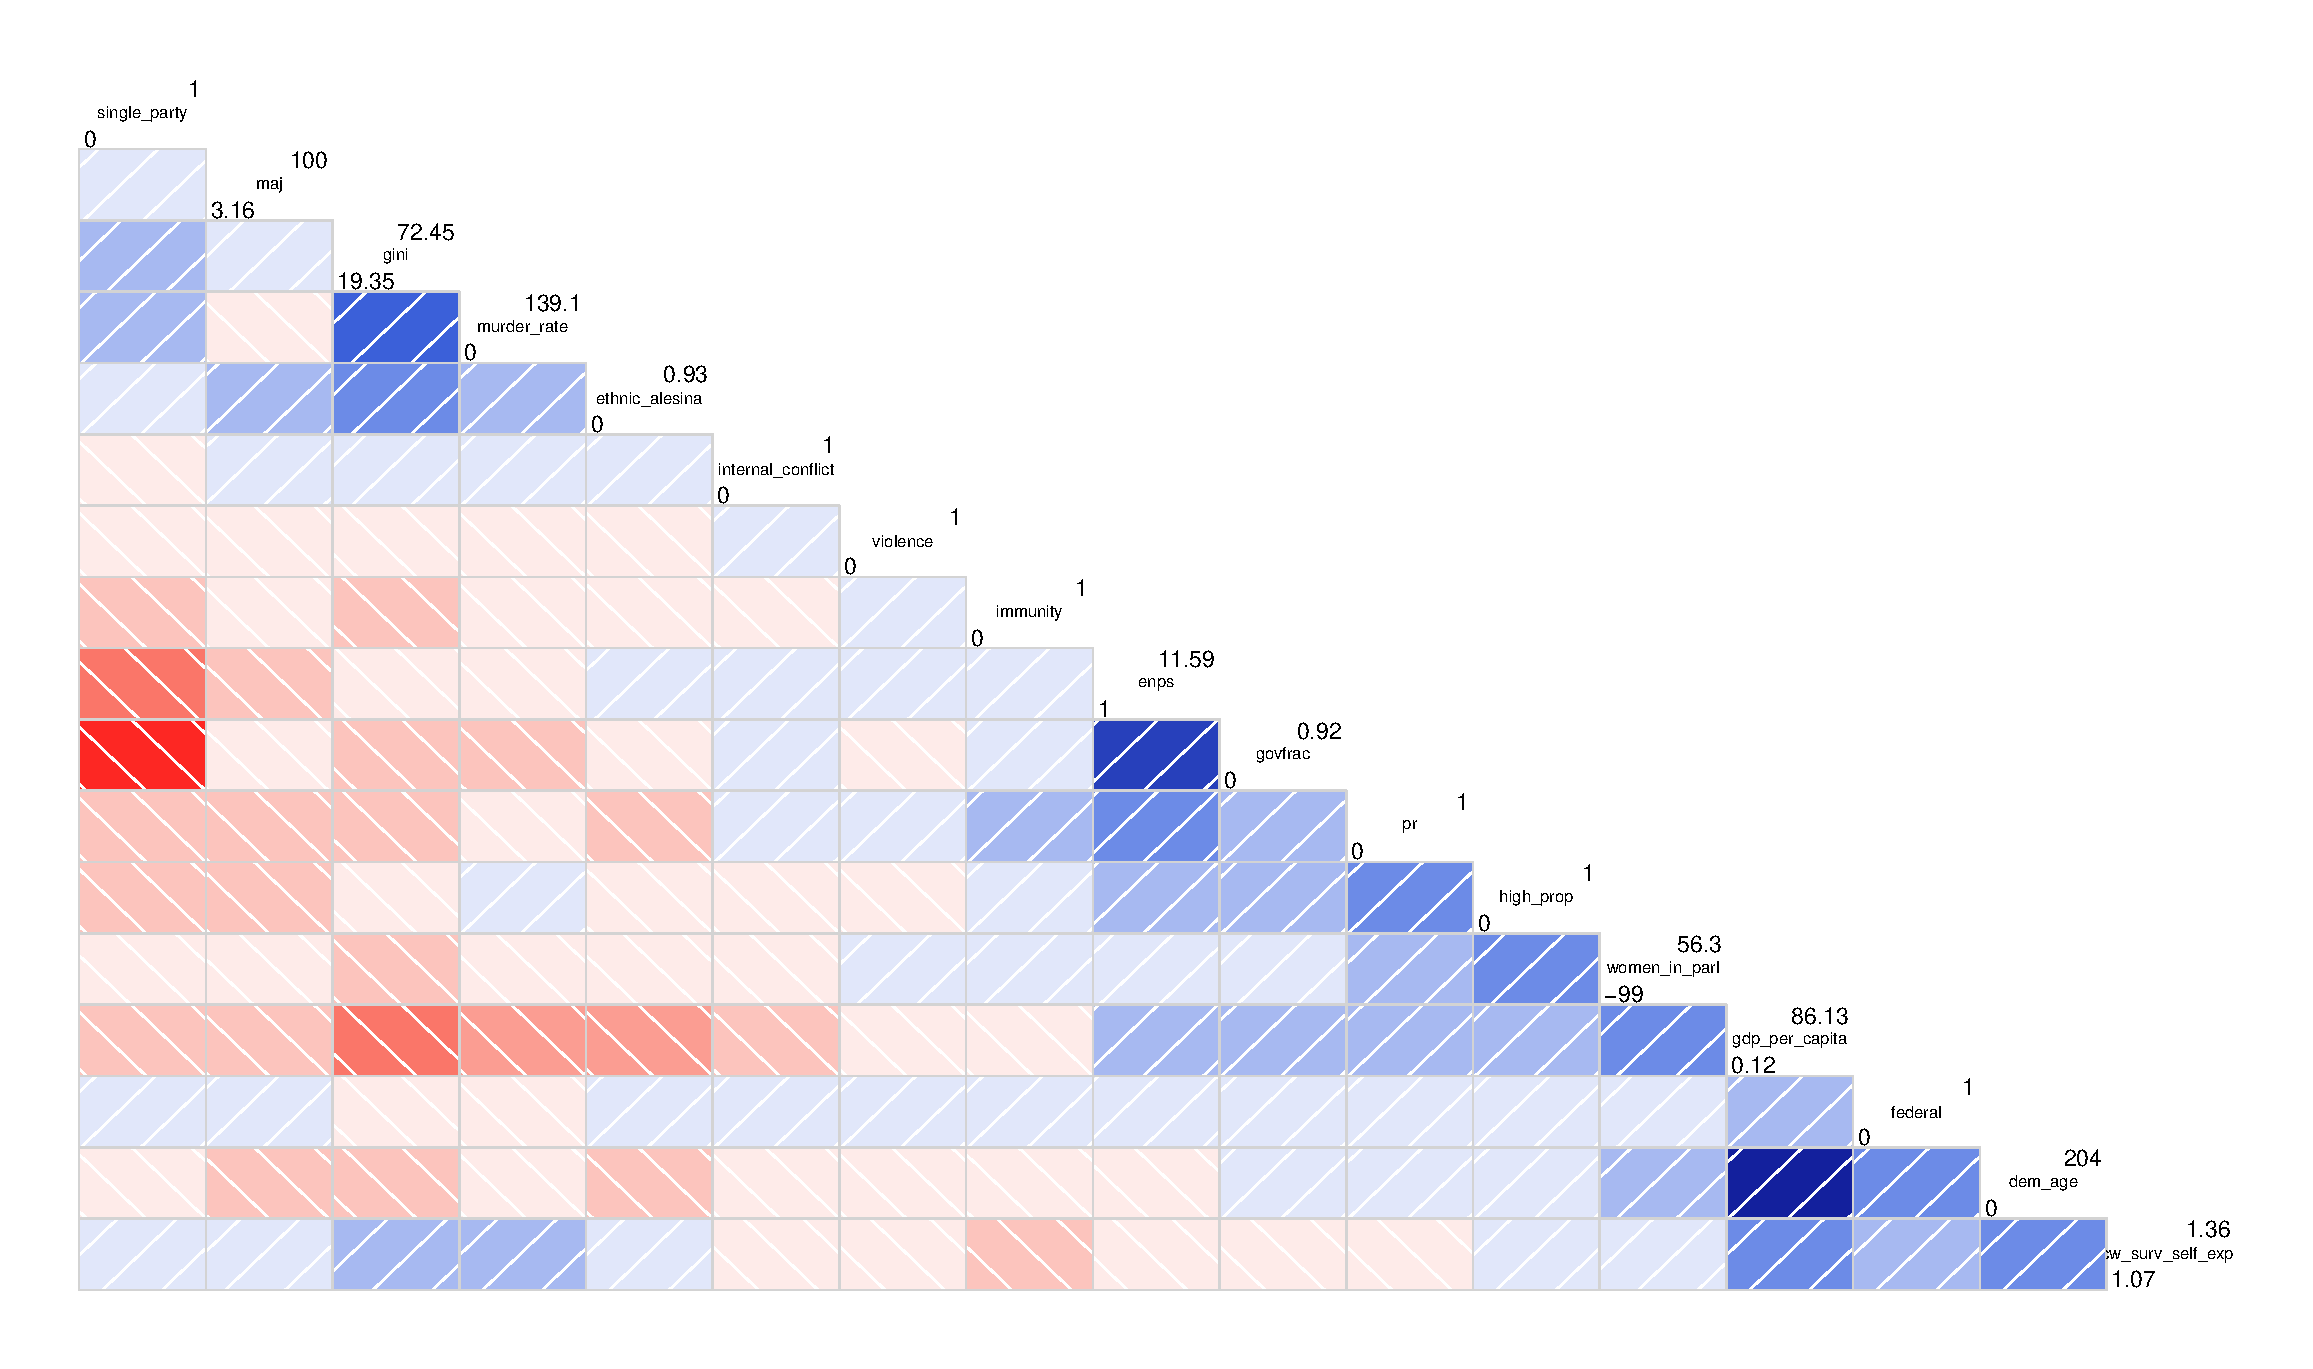
\includegraphics[width = \textwidth]{corrScatter.pdf}
    %%% corScatter not created every compile to save time %%%
%<<corScatter>>=

%    library(corrgram)

%    ### Create data set with variables for corrgram
%    vars.corrgram <- c("violence", "system", "DemAge", "maj", "MajCat", "govfrac", "singleParty", "pr", "tenshort", "UDS", "polity2", "ethnicAlesina", "CWtrust", "CWsurvSelfExpr", "disproportionality", "gini", "GDPperCapita", "enps", "enpv", "federal", "immunity", "UNMurderRate")

%    # Subset elected legislature data
%    dem.corrData <- dem[vars.corrgram]

%    # Create corrgram
%    dem.corrgram <- corrgram(dem.corrData, order = TRUE, upper.panel = NULL, diag.panel = panel.minmax)

%@

    \end{center}
    \begin{singlespace}
        {\scriptsize{Redder squares indicate stronger negative bi-variate correlations. \\
        Bluer squares indicate stronger positive bi-variate correlations. \\
        Numbers in the diagonal squares indicate the minimum and maximum observed values of the variables in the sample.
        }}
    \end{singlespace}
\end{figure}
\end{landscape}

%%%%%%%%%%%%%%%%%%%%%% Figures End %%%%%%%%%%%%%%%%%%%%%%%%%%%%%%%%%%%%%%%%%%%%%

\bibliographystyle{apsr}
\bibliography{LegViolence}

\end{document}
